\chapter{Ap�ndice}\label{ape:a}

\begin{figure}[ht]
  \centering
  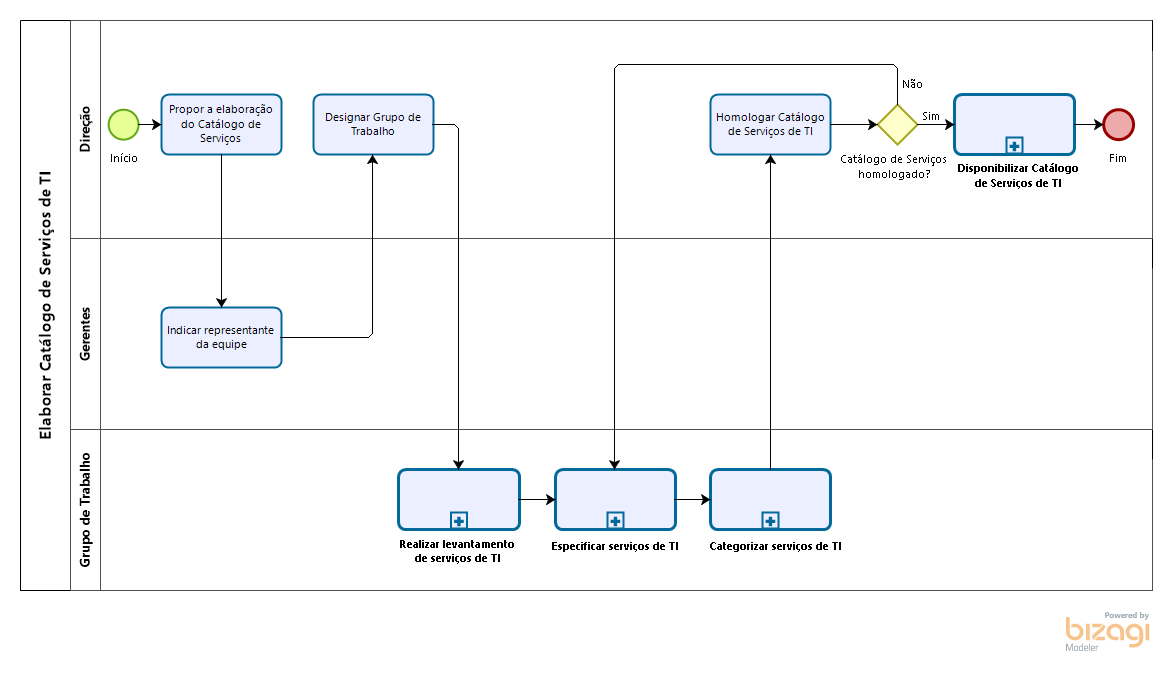
\includegraphics[width=\textwidth]{./fig/BPM_catalogo-servicos_elaboracao_resumido.png}
  \caption[]{Processo - Elaborar Cat�logo de Servi�os de TI.}
  \label{fig:elaborar-csti}
\end{figure}
\begin{figure}[!ht]
  \centering
  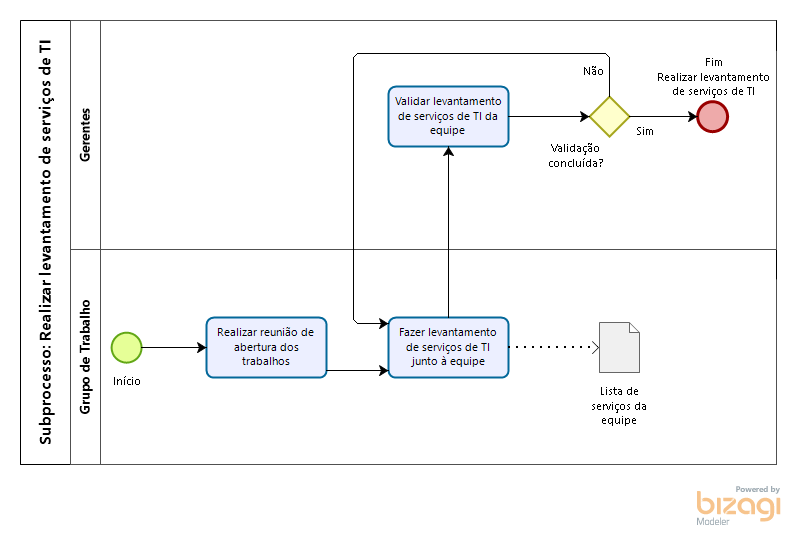
\includegraphics[width=\textwidth]{./fig/BPM_catalogo-servicos_sub-levantar-servicos.png}
  \caption[]{Subprocesso - Realizar levantamento de servi�os de TI.}
  \label{fig:levantamento-servicos-ti}
\end{figure}
\begin{figure}[!ht]
  \centering
  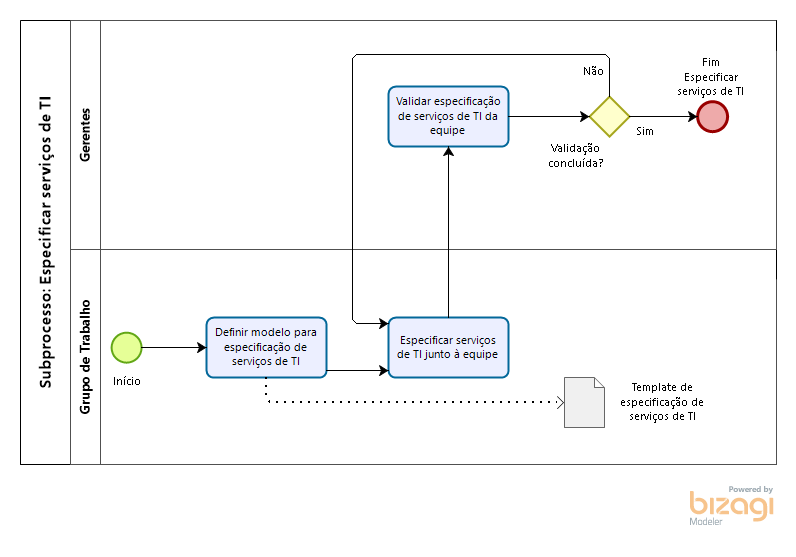
\includegraphics[width=\textwidth]{./fig/BPM_catalogo-servicos_sub-especificar-servicos.png}
  \caption[]{Subprocesso - Especificar servi�os de TI.}
  \label{fig:especificar-servicos-ti}
\end{figure}
\begin{figure}[!ht]
  \centering
  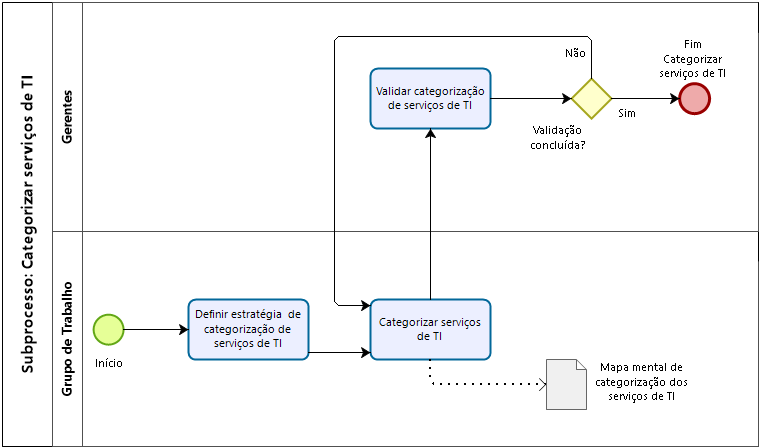
\includegraphics[width=\textwidth]{./fig/BPM_catalogo-servicos_sub-categorizar-servicos.png}
  \caption[]{Subprocesso - Categorizar servi�os de TI.}
  \label{fig:categorizar-servicos-ti}
\end{figure}

\chapter{Ap�ndice}\label{ape:b}

Aplica��o do ANS e do ANO na perspectiva do Cercomp e da sua divis�o de infraestrutura.

Anexo especifica��o de Servi�os de TI da categoria ``Servidores e Armazenamento'' preenchidos segunda a realidade do departamente de Infraestrutura do CERCOMP.
Os servi�os n�o contemplam informa��es ava�adas, parte C do formul�rio, mas pretende-se complement�-los com esses dados na medida que eles forem coletados da ferramenta de Ordem de Servi�o (OS).

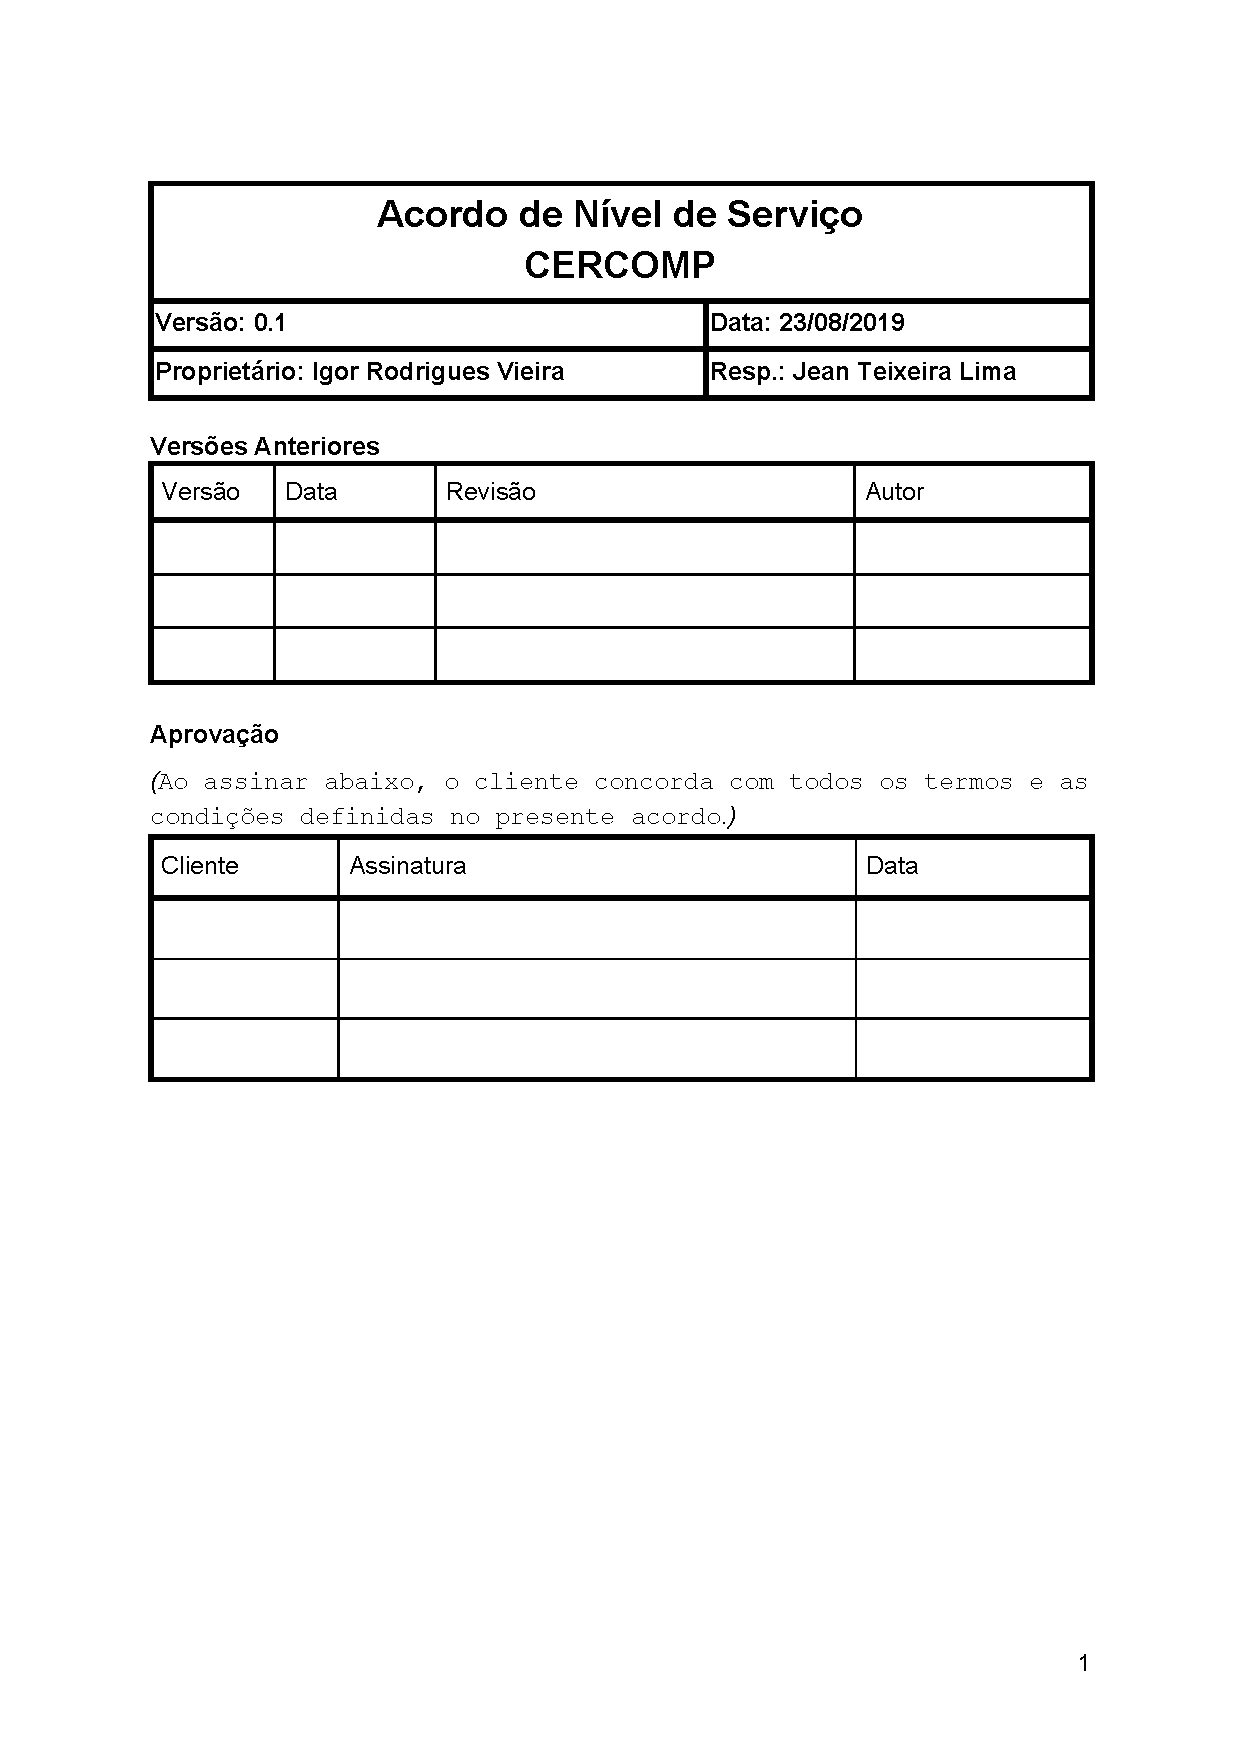
\includepdf[pages=-, pagecommand={}, width=\textwidth, frame=true]{./mods/ANS-CERCOMP_UFG.pdf}
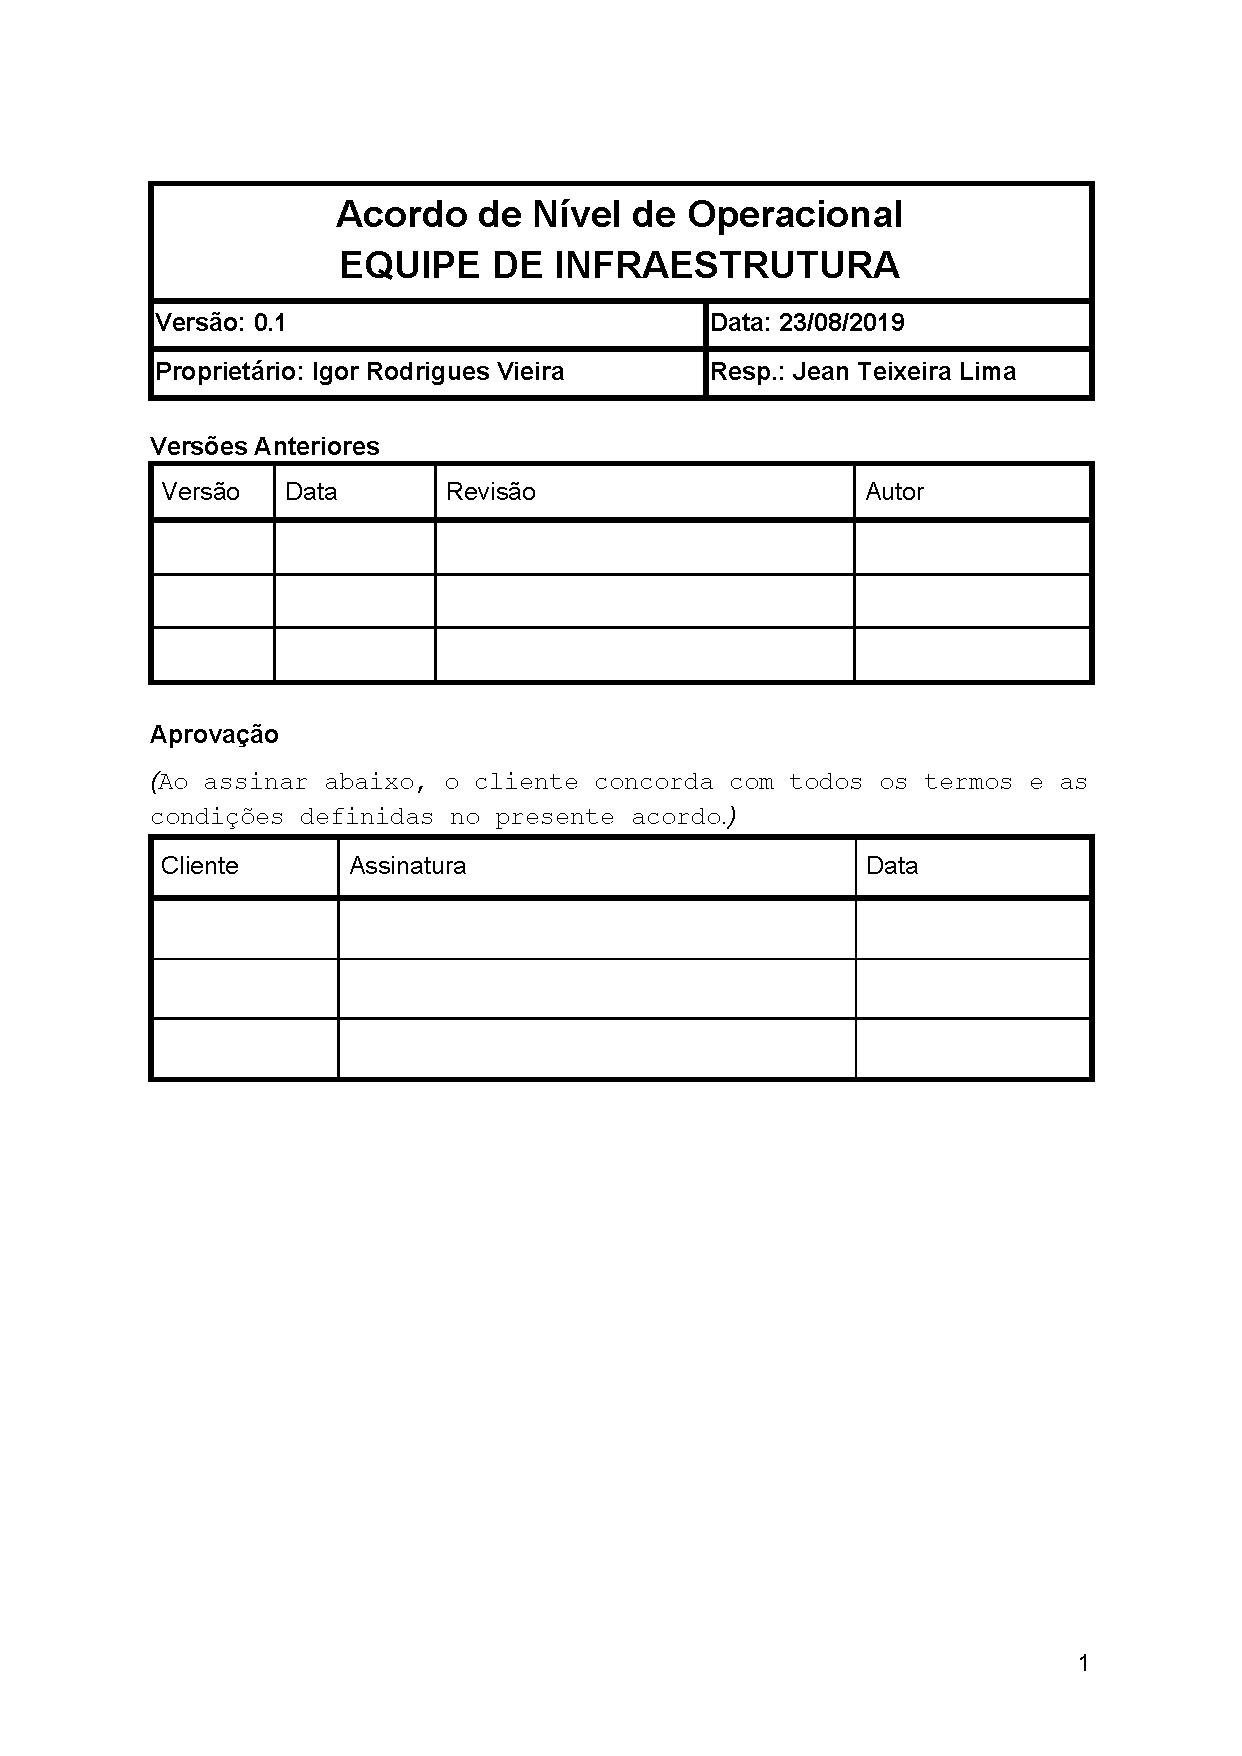
\includepdf[pages=-, pagecommand={}, width=\textwidth, frame=true]{./mods/ANO-Infra_Sistemas.pdf}
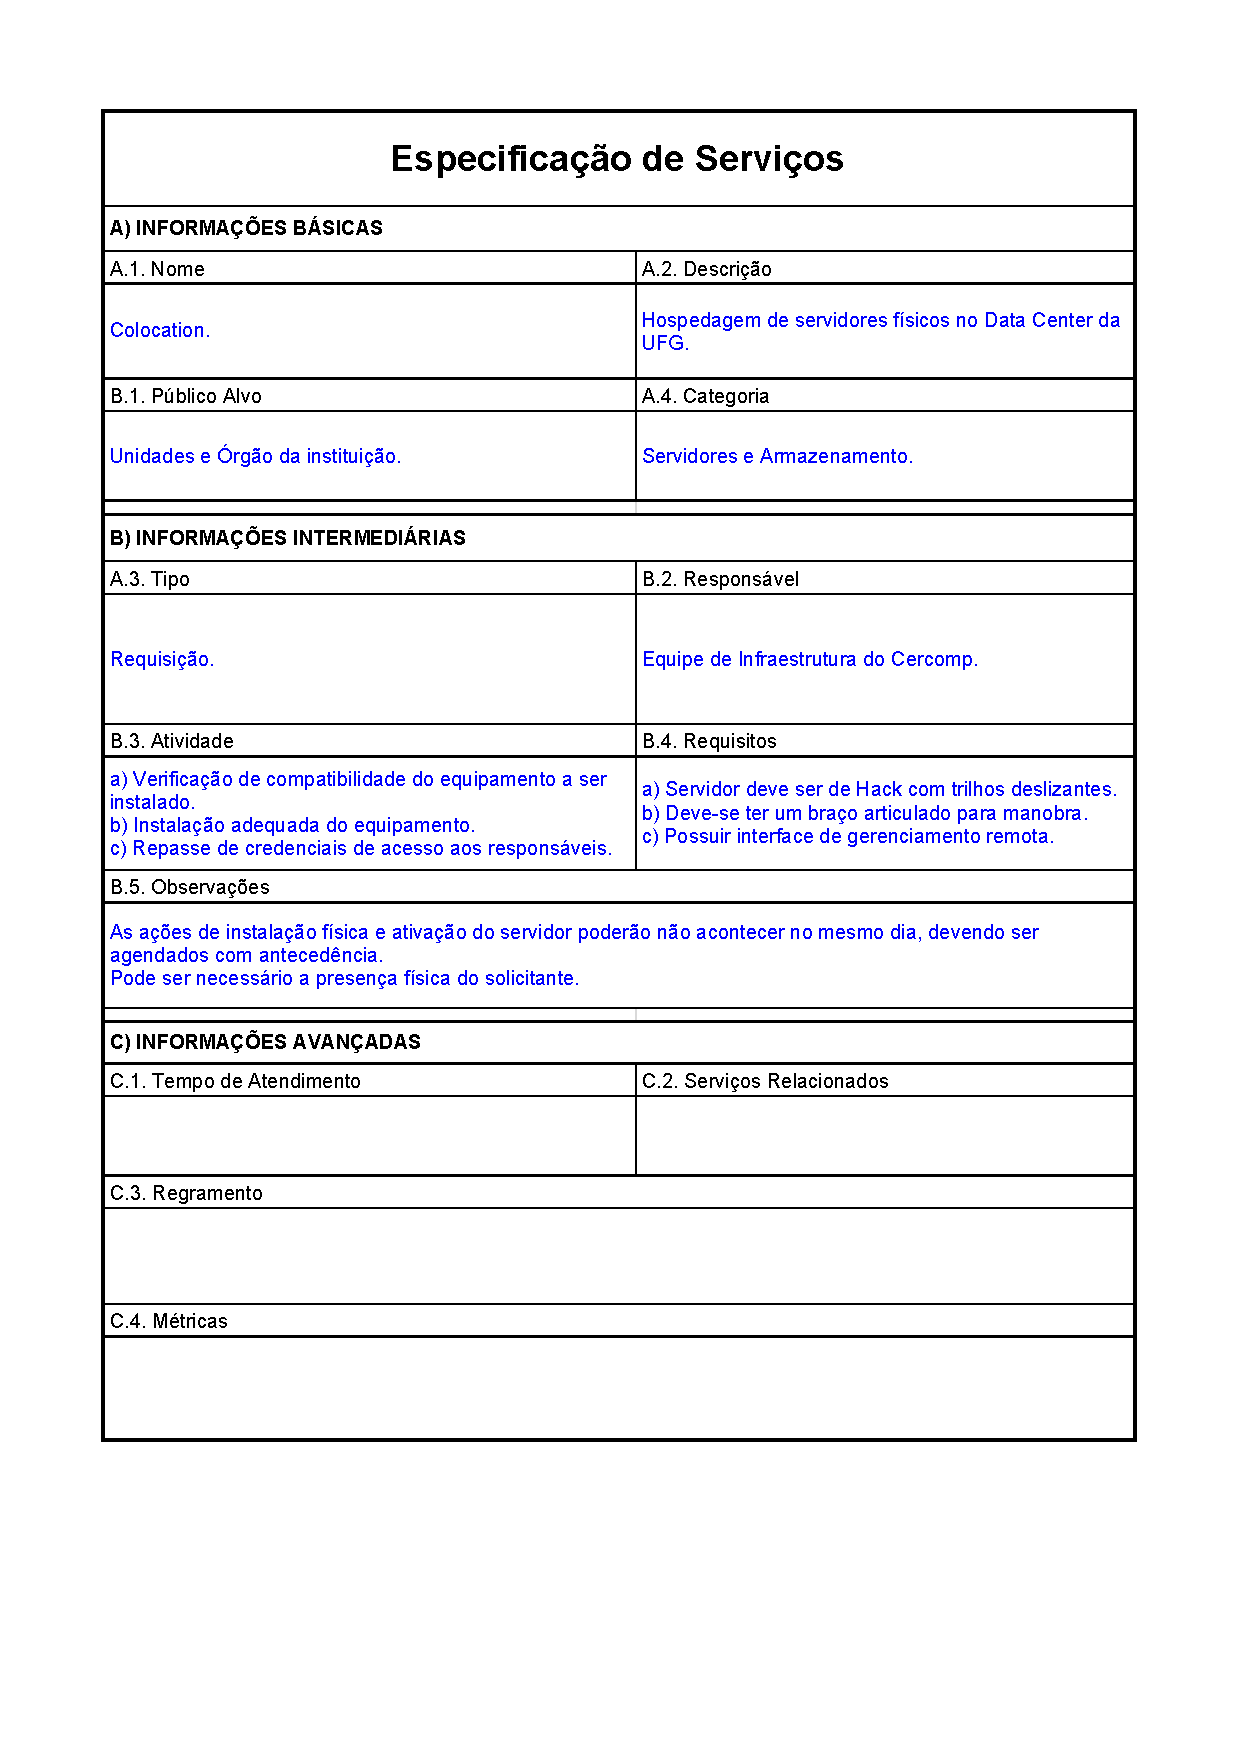
\includepdf[pages=-, pagecommand={}, width=\textwidth, frame=true]{./mods/especificacao-de-servicos_cat-servidores-e-armazenamento.pdf}

\chapter{Ap�ndice}\label{ape:c}

Anexo Modelo de Acordo de N�vel de Servi�o (ANS) e Modelo de Acordo de N�vel Operacional (ANO).

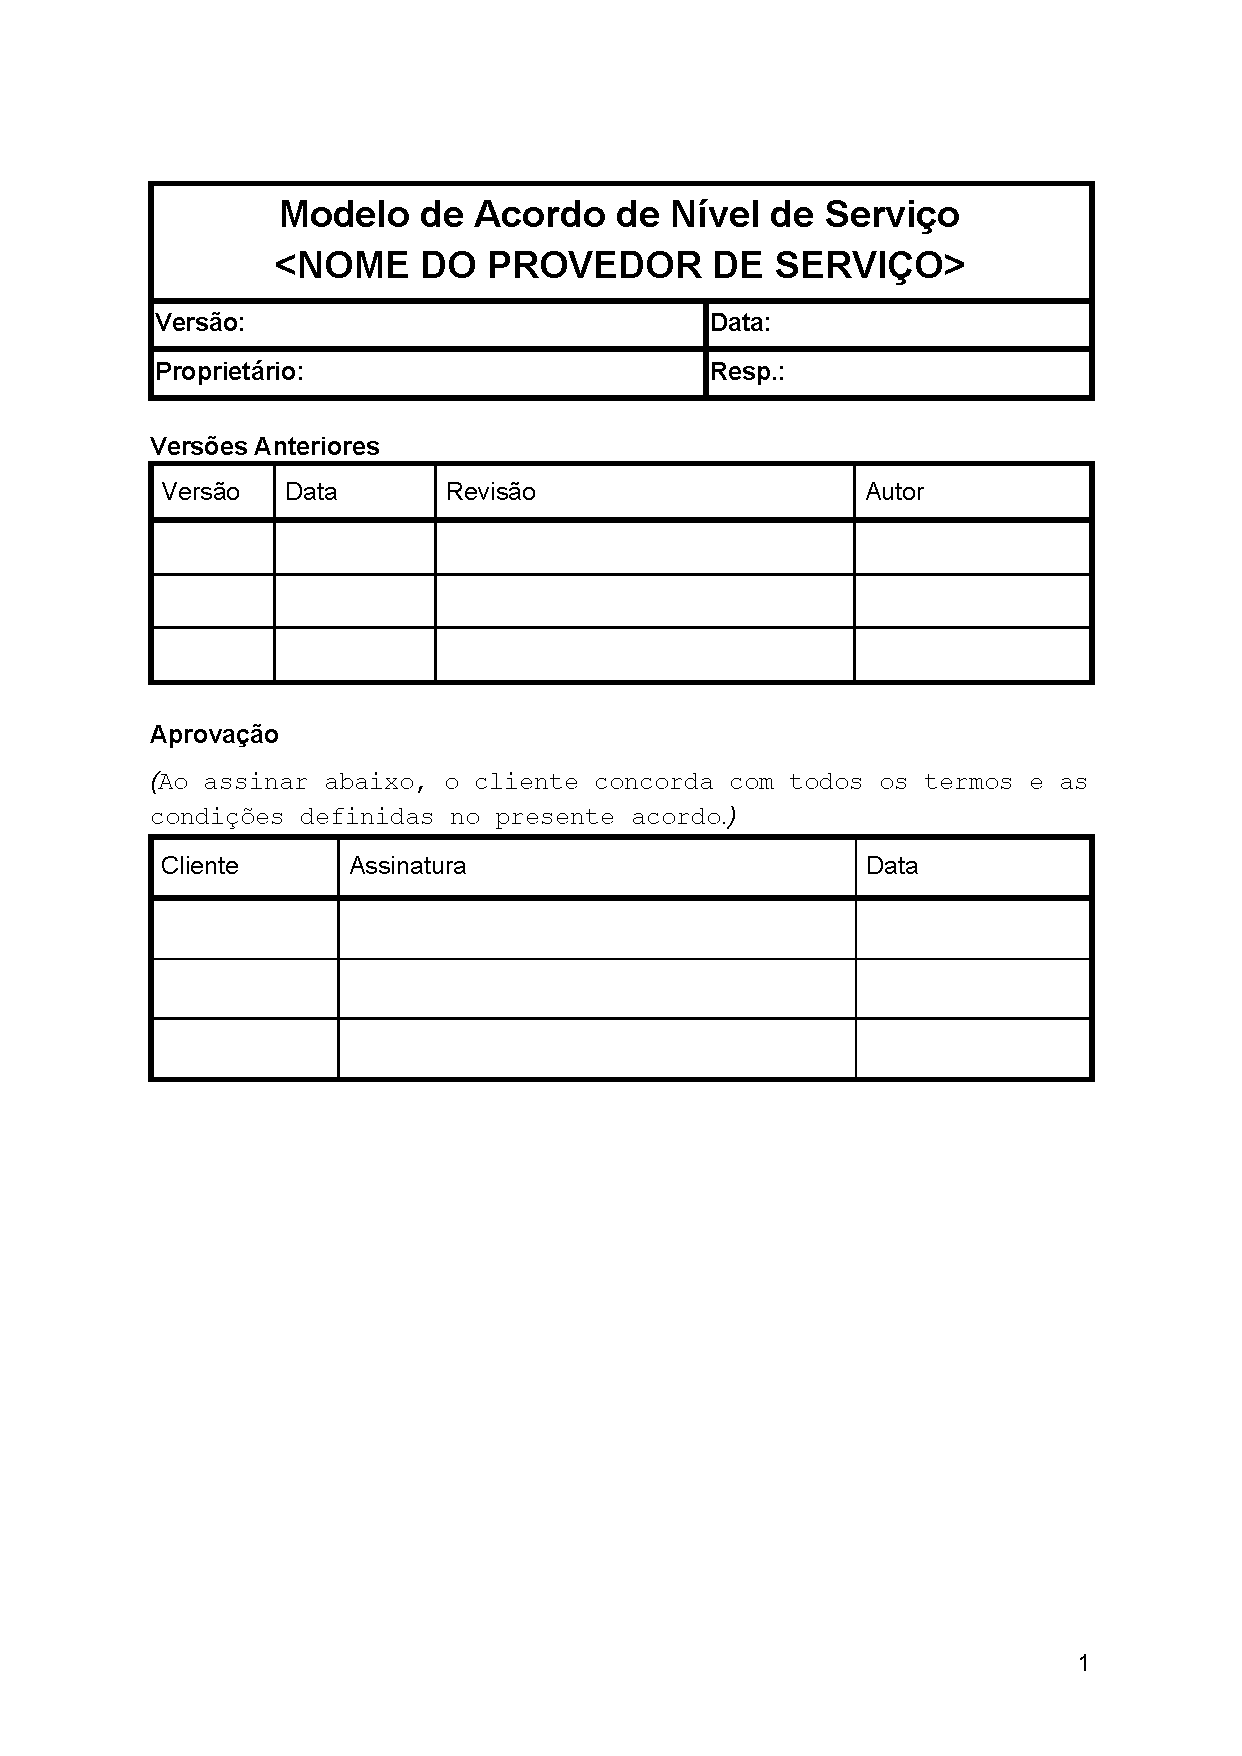
\includepdf[pages=-, pagecommand={}, width=\textwidth, frame=true]{./mods/modelo-de-ANS.pdf}
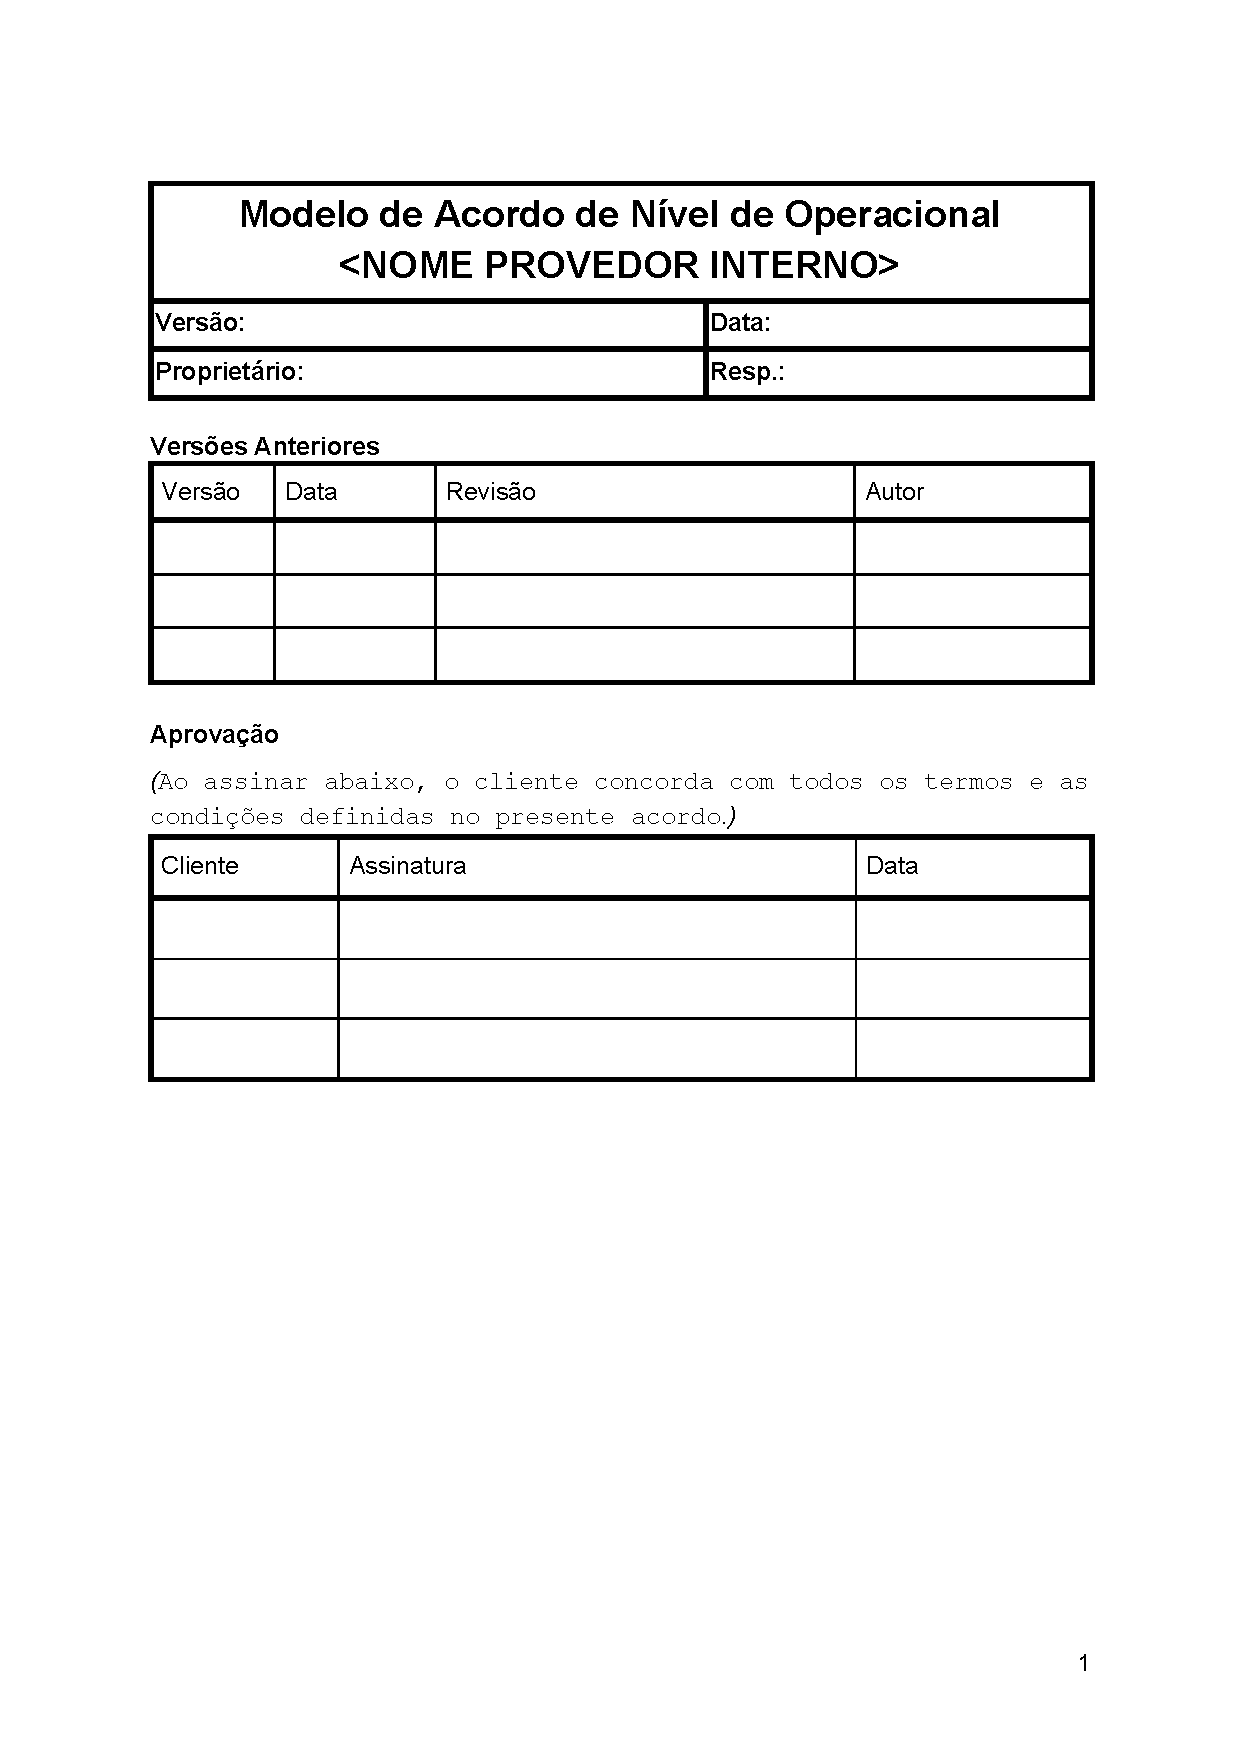
\includepdf[pages=-, pagecommand={}, width=\textwidth, frame=true]{./mods/modelo-de-ANO.pdf}
%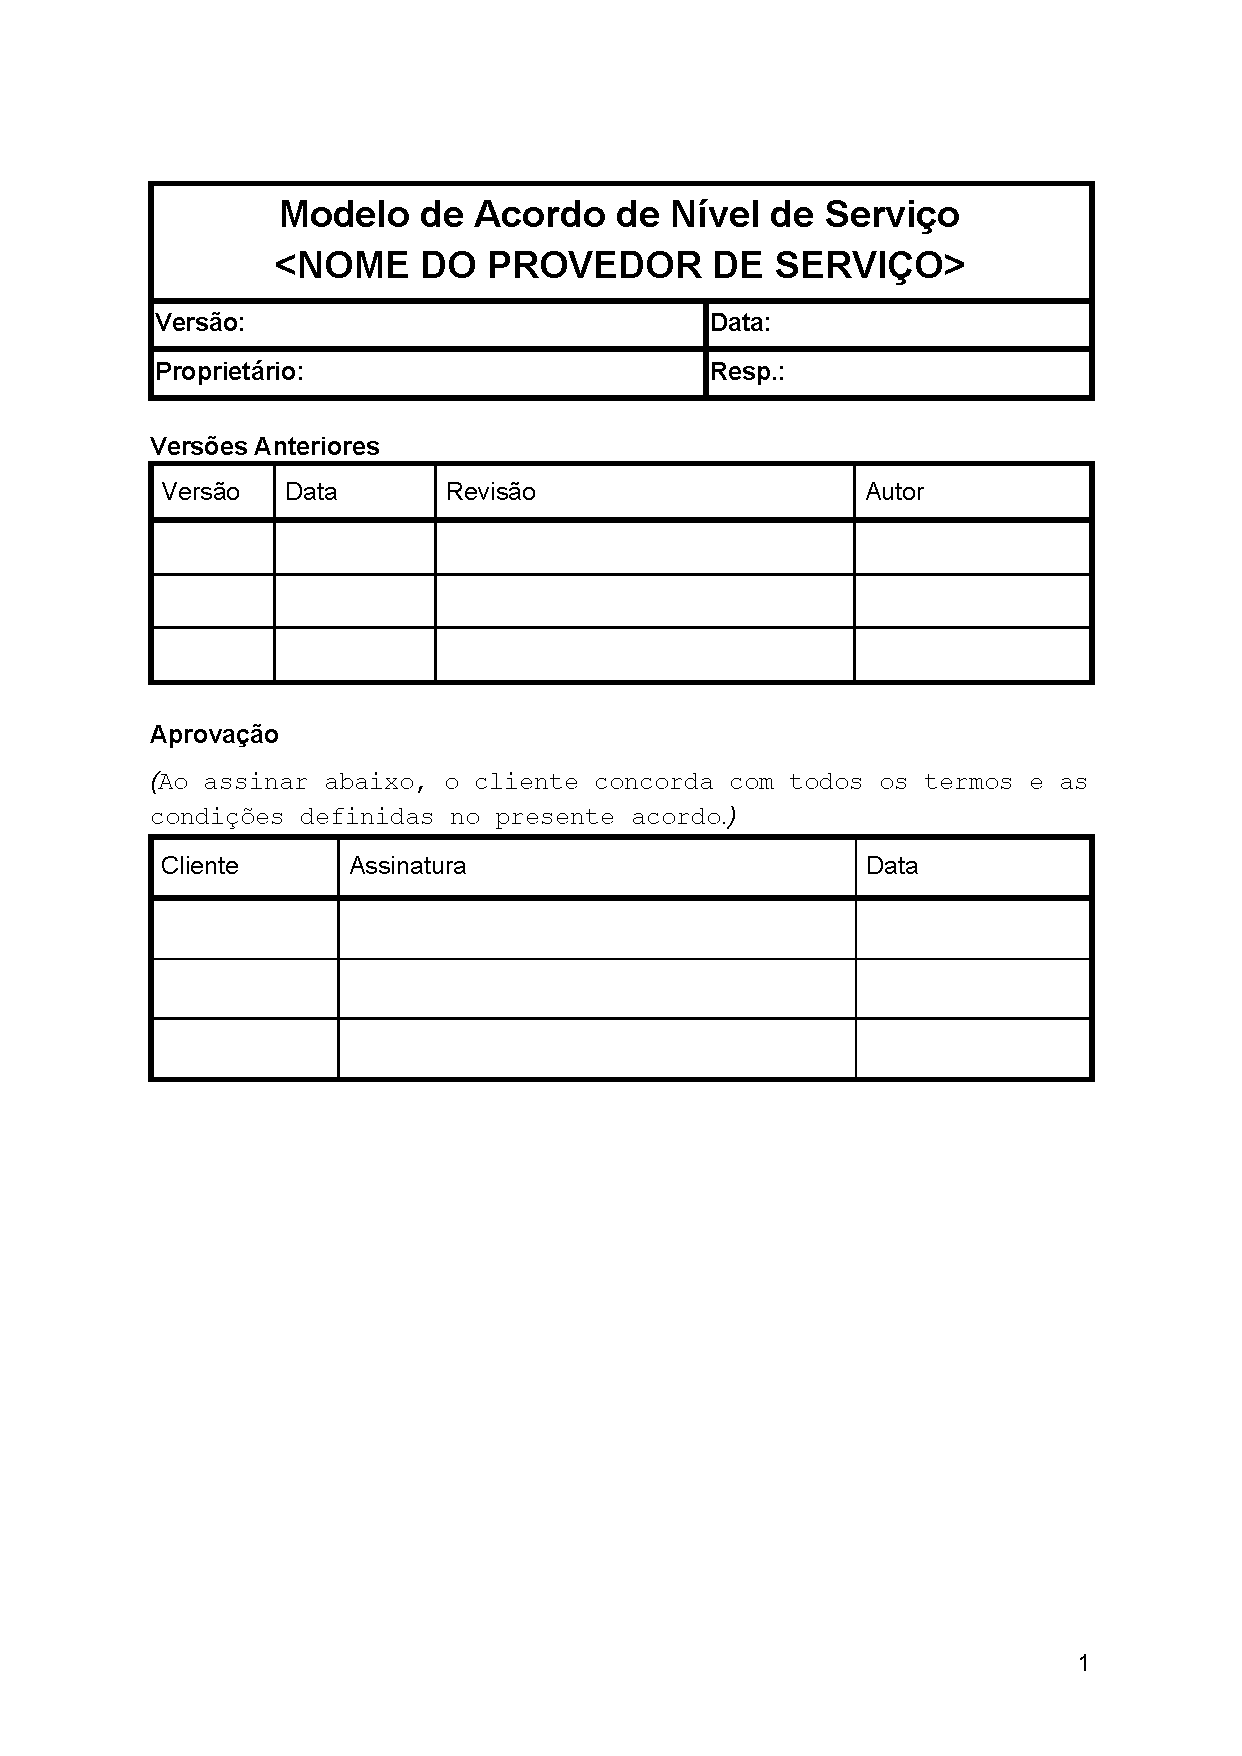
\includepdf[scale=1, offset={0 -70}]{./mods/modelo-de-ANS.pdf}

